\documentclass{suribt}
\title{ゲーム「2048」のプレイヤについて}
\author{金澤望生}
\eauthor{Kanazawa Nozomu}
\studentid{08-152021}
\supervisor{山口和紀 教授}
\handin{2018}{1}
\keywords{ゲームAI,機械学習}
\usepackage[dvipdfmx]{graphicx}
\usepackage{float}

\begin{document}
\maketitle

\frontmatter
\begin{abstract}
インターネットブラウザやスマートフォン上で遊ぶことのできるパズルゲーム「2048」をプレイするAIの改良を行った.改良には盤面上で最も大きな数のタイルが隅にあることを重視する独自のヒューリスティック「corner bonus」を使用した.(仮)
\end{abstract}

\tableofcontents

\mainmatter
\chapter{導入}
モチベーションや2048の基本ルール・指標について説明します.

\chapter{先行研究の紹介}
既存研究が使用している手法とプレイヤの成績について説明します.
\section{Szubert \& Jaskowski (2014)}
Szubert \& Jaskowskiは,TD学習を用いたプレイヤの訓練とnタプルネットワークを用いた価値関数の表現を組み合わせることによって,人間の知識やゲーム木探索を使用しないで十分強い2048プレイヤを実装することに成功した。
\subsection{TD学習}
TD学習の「TD」とはtemporal differenceの略であり,すなわち状態間における価値の差分を学習することによって学習器の訓練を行う手法である。2048にあてはめると,とある盤面$s'$の価値と,その盤面の1プレイ後の盤面$s'_{next}$の価値の差分を取り,これを現状定まっている$s'$に足し込んでいくことで訓練を行うことになる。TD学習にはさまざまな派生があるが,Szubert \& Jaskowskiが使用しているTD(0)学習は以下の式によって表現される:

\[
	V(s) ← V(s) + \alpha (r + V(s'') - V(s) )
\]

この式において,$V$は価値関数,$\alpha$は学習率,$r$は報酬である。学習率は計算された差分を価値関数の更新にどれほど反映するかを決定するパラメータである。

TD学習はTesauroによるバックギャモンへの適用でよく知られるようになり,碁やオセロ,チェスにおけるゲームAIの方策決定の手法として用いられるようになった。

\subsection{nタプルネットワーク}
TD学習によって盤面の評価とその学習を行うことができるが,盤面と評価値をどのように結びつけるかが問題になる。まず,2048で有り得るすべての盤面に対して評価値を与える1対1対応のルックアップテーブル(LUT)を作成することを考えると,2048で有り得る盤面の数は$(4 \times 4)^18 \approx 4.7 \times 10^21$と膨大な数になり,このようなLUTを計算機上で実装することは現実的に不可能である。

そこで,一部のマスの組み合わせによる「タプル」というクラスターを作成し,さらに複数のタプルを組み合わせることで盤面を表現する手法「nタプルネットワーク」を2048に導入することが,Szubert \& Jaskowskiによって提案された。たとえば,下記のようなnタプルネットワークを実装した場合,1つのゲーム内で保持すべき重みの数は860625であり,全ての有り得る盤面に対するLUTを保持するのに対して非常に少なくて済む。

\begin{figure}[H]
	\centering
	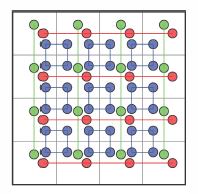
\includegraphics[width=5cm]{figure_001.png}
	\caption{nタプルネットワークの例}
\end{figure}

nタプルネットワークはBledsoe \& Browning (1959)によりパターン認識に用いられたのが最初の採用例である。ゲームAIの分野ではJaskowski (2014)によってオセロに適用され,一定の成果が得られた。

\chapter{本研究のアイディア}
本研究で導入しようとしている手法のアイディアについて説明します.

\chapter{提案と実装}
前章で説明したアイディアの具体的な提案とその実装方法を説明します.

\chapter{実験}
提案したアイディアの実験結果と既存研究の実験結果を比較します.

\chapter{考察と結論}
実験結果をもとに,結果の考察を行い,本研究をまとめます.

\backmatter
\chapter{謝辞}
謝辞を書きます.

\begin{thebibliography}{}
 \bibitem{}
 \bibitem{}
\end{thebibliography}

\appendix
\chapter{}
表やプログラムリストの掲載が必要になったらここに掲載します.

\end{document}
